\documentclass[11pt,a4paper]{article}
%Lorem Ipsum Einbindung
\usepackage{lipsum}

%Zeilenabstand
\linespread{1.5}
%graphics
\usepackage{graphicx}
\usepackage[margin=01in,includefoot]{geometry}
\usepackage{}
\usepackage{fancyhdr}
\usepackage{float}
%Einbindung Titelblatt mit PDF - Paket
\usepackage{pdfpages}

%Kopf, Fusszeilen
\pagestyle{fancy}
\fancyfoot{}
\fancyhead{}
\fancyfoot[R]{\thepage\ }
\usepackage{geometry}
\geometry{tmargin=25mm,bmargin=20mm,lmargin=27mm,rmargin=25mm}

%Literaturverzeichnis und Zitieren
\usepackage{apacite}
\bibliographystyle{apacite}
\usepackage{url}
\def\UrlBreaks{\do\/\do-}
\usepackage{nameref}

%URL nicht in anderer Schrift (z.B. Bibliografie)
\usepackage{url}
%Fussnoten am Ende der Seite
\usepackage[bottom]{footmisc}

\usepackage{amsmath}
\usepackage{hyperref}
\usepackage{graphicx} %Package f�r Grafiken
\usepackage{subfig} % Package f�r mehrere Grafiken nebeneinander
%\DeclareMathOperator{\atantwo}{atan2}

\begin{document}

%Titelseite Einbindung PDF
\begin {titlepage}
%\includepdf{Titelblatt}
\end {titlepage}
\newpage


\section*{Abstract} \label{sec:Abstract}

In dieser Arbeit werden die Notwendigkeit, wie auch Gegenargumente einer globalen Finanzmarktregulierung analysiert und diskutiert. Die nachfolgende Argumentation st\"utzt sich auf ein intensives Literaturstudium. Aus der Untersuchung wird ersichtlich, dass trotz zus\"atzlicher Kosten, einer steigenden Sicherheit und der Gefahr von regulatorischer Arbitrage eine globale Finanzmarktregulierung einen positiven Einfluss auf die Weltwirtschaft haben k\"onnte. Denn falsche Anreize und starke negative Externalit\"aten, wie explizite und implizite Staatsgarantien, aber auch die Gefahr einer Kreditklemme, verzerren den Markt und f\"uhren schliesslich zu weniger Wohlstand.

\newpage
%Inhaltsverzeichnis
\tableofcontents
\newpage
%Tabellen- und Abbildungsverzeichnis, plus hinzuf\"ugen zu TOC, ohne Nummerierung
\listoffigures
\addcontentsline{toc}{section}{\listfigurename}
\vspace{12cm}
Aufgrund der besseren Lesbarkeit und der Einfachheit halber wird in der vorliegenden Arbeit nur die m�nnliche Form verwendet. Die weibliche Form ist selbstverst�ndlich immer miteingeschlossen.

\newpage
\section{Einleitung}\label{sec:Einleitung}
\begin{quotation}
``Regulation is necessary, particularly in a sector, like the banking sector, which exposes countries and people to a risk'' \cite{lagarde2018}.
\end{quotation}

\section{Data Cleaning and Preparation}

\section{New York Inspection Data}

The main dataset for our project is retrieved from the \href{https://data.ny.gov/Economic-Development/Retail-Food-Store-Inspections-Current-Ratings/d6dy-3h7r}{official site of the State of New York}. It contains a total of 28'300 A to C ratings from of food store inspections. When we downloaded the data on the XXX it has been the version of June 26, 2019 with observations from March 2018 to March 2019.\\
\\
The data published by the state of New York includes not only a list of all the food ratings of different shops but also part of the history of the inspection grade development. This means the same shops could appear several times with different issues. To avoid the problem of having the identical shop more than one time we ordered the dataset ascending to the inspection date. Considering only the newest entry of every shop would have led to a bias regarding the hygiene grade because the bad graded shops improved themselves. Thus we decided to only take in account the oldest entry of every shop. This resulted in a data frame of around 7500 unique shops in the city of New York.
\\
Additionally, the data set reveals not only the shops trade name but also its owner. This enabled us to identify if the shop is part of a chain. We added this parameter beside to the number of shops which belong to the specific chain. It seems possible to have an impact on the hygiene grade if the shop is part of a bigger chain. 
\\
We will predict the food store inspection ratings from this dataset with different covariates whose derivation is outlined in the following sections.

\section{Chain Information}

\section{Spatial Data}



\section{Subway Data}

In a next step, we amend our New York City inspection data with location information of subway stations. We use again \href{https://data.ny.gov/Transportation/NYC-Transit-Subway-Entrance-And-Exit-Data/i9wp-a4ja}{an official dataset provided by the State of New York}. The dataset contains the location of every subway entrance and its corresponding station. We are only interested in the station. Therefore, we remove all duplicates of stations with multiple entrances and then use again the Haversine Formula to find the distance of the closest station to every shop.

\subsection{Google web scraper}

While doing research to find datasets with regards to food inspections we decided to gather more information from webpages. The reviews from customers, written on google places, could give us information about how individual persons have experienced their visit to the specific food shop. In order to gather this information from the internet we set up a web scraper. We used the package \textit{RSelenium} to execute an automated google search for all the observations. This included a lot of trial and error due to unforeseen changes of the xPaths and other errors. Most of the errors only showed up in the middle of the scraping process, which had a duration of about 24 hours for all the food shops. Therefore, it was only possible to adjust the function after the script run during the night. This resulted in a lot of waiting and adjusting but finally the data was scraped successfully. Nonetheless the scraped data was not in a useable format yet. After tidying and joining the data to the original dataset it was ready to be used. \\

A brief analysis of the dataset revealed the incompleteness of the ratings. Approximately 40\% of the shops don't have an entry in google places and thus neither rating. After a lot of discussion on how to handle the problem we agreed on using the number of reviews as a parameter of the internet popularity. 



\subsection{Airbnb data and spatial analysis}

In order to acquire additional data and parameters on the location of the shops, we integrated data from Airbnb (average price and number of rooms). To join the original and the airbnb data frames a matching key is needed. Regarding the dataset only longitude and latitude were available. Therefore we used the above mentioned spatial data to assign the respective parameter to the ZIP codes in New York. Thereafter we grouped the data by ZIP code, calculated the respective means and counts and added it to the new data frame.


\section{Random Forest Analysis}

We decided to use the random forest to have a model with a typically good performance but relatively little tuning requirements. Additionally, the structure of the dataset according to the correlation matrix, seemed rather complex and not linear. Tree models normally outperform linear models in these situations \cite{James}[S. 314] In order to address the problem of class imbalances, the random forest model is built up on bagging mentioned above. Beside several similarities the methodology differs in the following points:
\begin{enumerate}
\item Evaluate the different tuning parameter (minimal node size, split rule, number of variables available for splitting at each tree node) in Cross-Validation
\item Calculate the different errors for all the bagging samples
\item Choose the model based on the best performance of the tuning parameters
\item Apply the majority vote to the trained optimal model to get the final predictions
\end{enumerate}

Although there is normally only little tuning required, the evaluation of tuning parameter is computationally very intensive due to an exponential rise of possible combinations with every new tuning parameter. Therefore we were restricted to a smaller selection of possible tuning grid and only used 40 different combinations. The following graph shows the progress in the model selection process. \\

\begin{figure}[H]
\centering
\captionof{figure}{Tuning progress in random forest} \label{rf_tuning}

       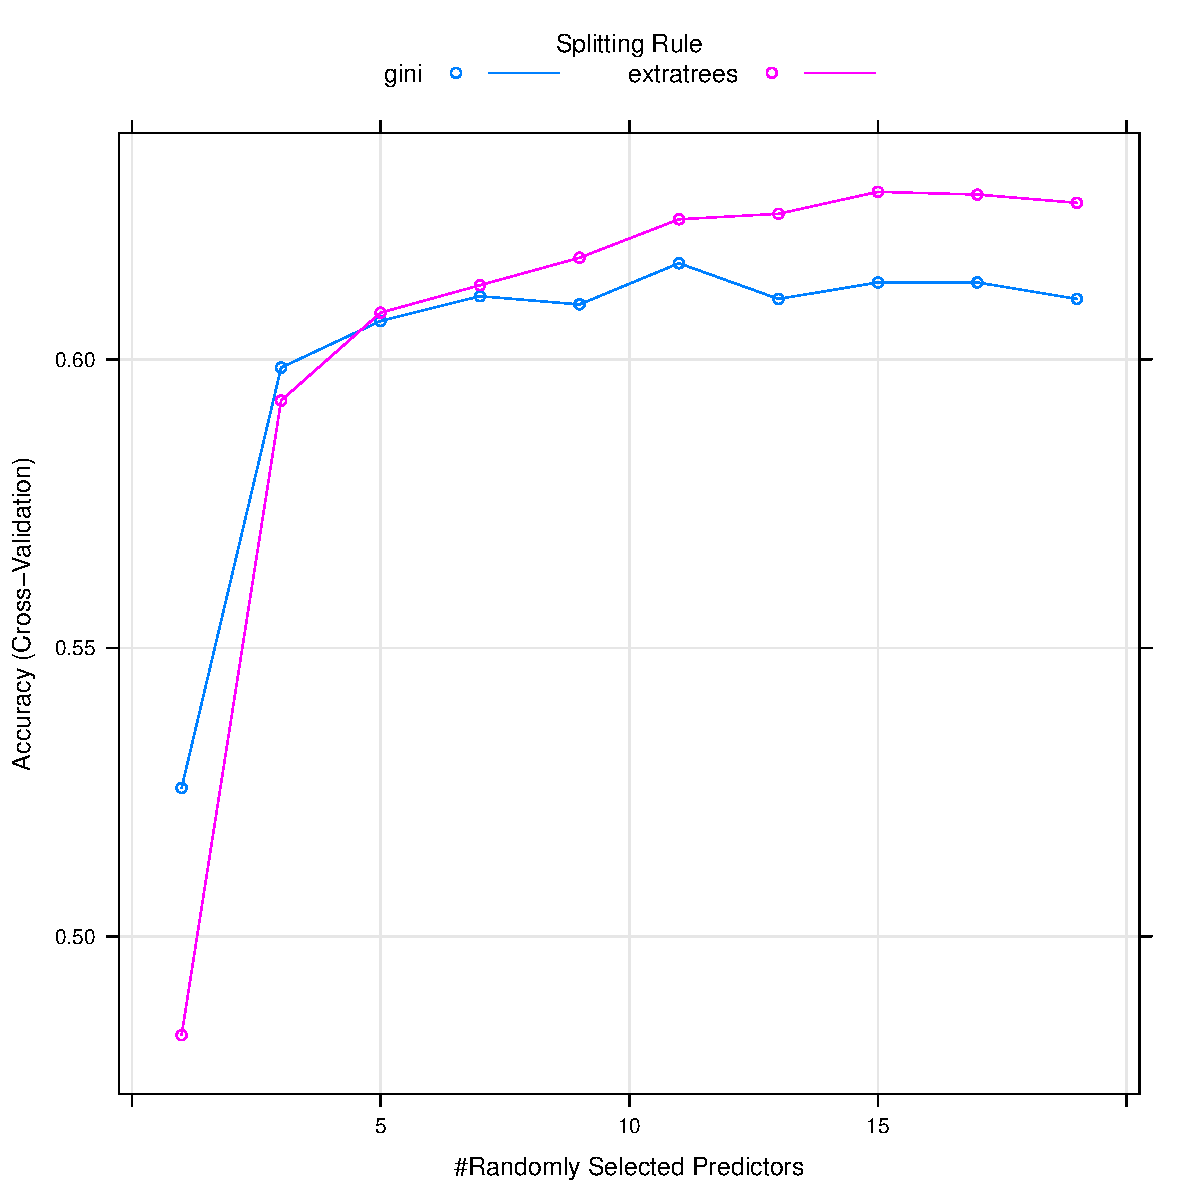
\includegraphics[width=0.5\textwidth]{Plots/rf_progress.pdf}
 

\end{figure}

The importance of the variables can be shown in figure \ref{var_importance}

\begin{figure}[H]
\centering
\captionof{figure}{A variable importance plot for the selected parameters. Variable importance is computed using the mean decrease in Gini index and expressed relative to maximum} \label{var_importance}

       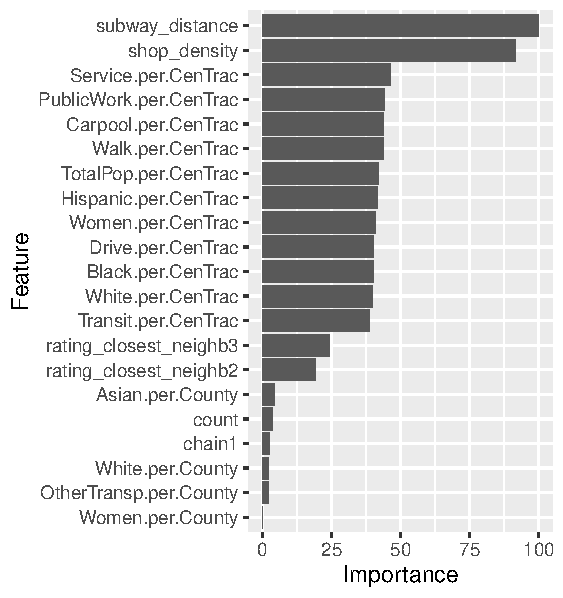
\includegraphics[width=0.5\textwidth]{Plots/var_importance.pdf}
 

\end{figure}
%overbagging

\begin{table}[ht]
\centering
\begin{tabular}{rllr}
  \hline
 & Var1 & Var2 & Freq \\ 
  \hline
1 & A & A & 4327 \\ 
  2 & B & A &   0 \\ 
  3 & C & A &   2 \\ 
  4 & A & B &   0 \\ 
  5 & B & B & 661 \\ 
  6 & C & B &   0 \\ 
  7 & A & C &   0 \\ 
  8 & B & C &   0 \\ 
  9 & C & C & 1859 \\ 
   \hline
\end{tabular}
\end{table}

%Underbagging
\begin{table}[ht]
\centering
\begin{tabular}{rllr}
  \hline
 & Var1 & Var2 & Freq \\ 
  \hline
1 & A & A & 2551 \\ 
  2 & B & A &   0 \\ 
  3 & C & A & 224 \\ 
  4 & A & B & 829 \\ 
  5 & B & B & 661 \\ 
  6 & C & B & 233 \\ 
  7 & A & C & 947 \\ 
  8 & B & C &   0 \\ 
  9 & C & C & 1404 \\ 
   \hline
\end{tabular}
\end{table}

\label{pred-matrix}
\captionof{table}{Prediction Matrices of Different Estimated Models}
\begin{center}
\begin{small}
\begin{tabular}{ l | c c c}
\multicolumn{4}{c}{QDA} \\
\hline
Obs / \\ Pred & A & B &C \\
\hline
A &2839 & 462 & 1164 \\
B &1260 & 173 & 594 \\
C &228 & 26 & 103 \\
\hline
\end{tabular}
\quad






\section{Gradient Boosting}

As a further method of tree based models we implemented extreme gradient boosting. It enables a better performance than random forest and provides more advanced tuning methods. The selected parameters have XXX different combinations which have to be evaluated. The current approach with a full hyper grid search is computationally very intensive and takes several days with an ordinary computer. Another possibility is to use a random discrete search which does not test all combinations but a sample of it with a stopping parameter. Thus this would have meant to implement another package and due to time restrictions was entirely finished.

\section{Zusammenfassung und Diskussion der Resultate} \label{sec:Diskussion}

In dieser Arbeit wurden die Notwendigkeit und allf\"allige Gegenargumente einer globalen Finanzmarktregulierung untersucht. 
%Literaturverzeichnis
\urlstyle{rm}

\newpage
\bibliography{bib}
\newpage

\textbf{Eigenst\"andigkeitserkl\"arung und Zeichenzahl}\\
\\
�Ich erkl\"are hiermit, 
\begin{itemize}
\item[- ]dass ich die vorliegende Arbeit selbstst�ndig, ohne fremde Hilfe (Lektorat, �bersetzungsdienstleister etc.) und ohne Verwendung anderer als der angegeben Hilfsmittel verfasst habe;
\item[- ]dass ich s�mtliche verwendeten Quellen erw�hnt und gem�ss g�ngigen wissenschaftlichen Zitierregeln korrekt zitiert habe;
\item[- ]dass das Thema, die Arbeit oder Teile davon nicht bereits Gegenstand eines Leistungsnachweises einer anderen Veranstaltung oder Kurses waren;
\item[- ]dass ich ohne schriftliche Zustimmung der Universit�t keine Kopien dieser Arbeit an Dritte
aush�ndigen oder ver�ffentlichen werde, wenn ein direkter Bezug zur Universit�t St.Gallen
oder ihrer Dozierenden hergestellt werden kann;
\item[- ]dass ich mir bewusst bin, dass meine Arbeit elektronisch auf Plagiate �berpr�ft werden kann
und ich hiermit der Universit�t St.Gallen laut Pr�fungsordnung das Urheberrecht soweit einr�ume, wie es f�r die Verwaltungshandlungen notwendig ist;
\item[- ]dass ich mir bewusst bin, dass die Universit�t einen Verstoss gegen diese Eigenst�ndigkeitserkl�rung sowie insbesondere die Inanspruchnahme eines Ghostwriter-Service verfolgt und dass daraus disziplinarische wie auch strafrechtliche Folgen resultieren k�nnen, welche zum Ausschluss von der Universit�t resp. zu einer sp�teren Titelaberkennung f�hren k�nnen�
\end{itemize}

(Zeichen: 44'978)
\end{document}